\documentclass[11pt,a4paper]{article}

% Basic required LaTeX packages
\usepackage[utf8]{inputenc}
\usepackage[T1]{fontenc}
\usepackage{microtype} % Improves typography
\usepackage{graphicx} % For including graphics
\usepackage{booktabs} % For professional looking tables
\usepackage{float}

% Math packages
\usepackage{amsmath} % Essential for math environments
\usepackage{amssymb} % Additional math symbols
\usepackage{amsthm}  % Theorem environments
\usepackage{mathtools} % Extensions to amsmath

% Define Thms
\newtheorem{theorem}{Theorem}
\newtheorem{definition}[theorem]{Definition}
\newtheorem{corollary}{Corollary}[theorem]
\newtheorem{lemma}[theorem]{Lemma}

% Physics package
\usepackage{physics} % Simplifies many physics notations

% For better handling of hyperlinks
\usepackage[colorlinks=true, allcolors=blue]{hyperref}

% For bibliography
\usepackage{cite} % If you are using BibTeX

% For better captioning
\usepackage{caption}
\usepackage{subcaption}

% For multiple columns
\usepackage{multicol} 
\usepackage{multirow}

% For creating lists
\usepackage{enumitem}

% For improved tables
\usepackage{tabularx}

% Colours
\usepackage{xcolor}
\title{MCM/C}
\begin{document}
	\maketitle
	\tableofcontents
	
	\section{Background Information}	
	The 2023 Wimbledon Championships marked a significant event in the world of tennis, particularly in the Gentlemen's Singles category. One of the most notable matches was the final between the young Spanish sensation, 20-year-old Carlos Alcaraz, and the seasoned champion, 36-year-old Novak Djokovic. In a surprising turn of events, Alcaraz defeated Djokovic, ending the latter's impressive winning streak at Wimbledon since 2013. This match stood out not just for its outcome but also for its dramatic shifts in momentum, a concept often discussed in sports but hard to quantify. Throughout the match, both players exhibited periods of dominance, with the advantage oscillating between them in an unpredictable manner. This intriguing match, along with other games from the tournament, provides a rich dataset to explore the elusive concept of momentum in tennis and its impact on match outcomes.
	
	Momentum in sports has been studied by many scholars in various fields. Some aim to quantify momentum from a statisitical point of view, while others try to explain it from a sports psychological point of view. All fields are equally valid. However, our team will build a mathematical model to explain and answer the following questions:
	
	\begin{itemize}
		\item Create a model to capture the flow of play in tennis matches, identifying the player performing better at any given time and the extent of their advantage.
		\item Provide a visualization based on your model to depict the match flow.
		\item Use our model to evaluate the claim: "swings in a tennis match are random, as opposed to being influenced by momentum."
		\item Develop a model that predicts when the flow of play is about to change. Identify factors that might be related to these shifts.
		\item Test your model on other matches to evaluate its effectiveness and generalizability.
		\item Produce a report (max 25 pages) with your findings. Include a memo summarizing results and advice for coaches regarding momentum and preparation for matches.
	\end{itemize}
	
	\subsection{Some Info on Tennis Scoring}
	\paragraph{Game}
	\begin{itemize}
		\item Each point won counts as one. 
		\item The first to score 4 points wins the game.
		\item At 3 points each, the score is 'Deuce.' From Deuce, a player must win by two points to win the game. 
		\item In international tennis, the scores of 0, 1, 2, and 3 points are represented by the English words Love, 15, 30, and 40, respectively.
	\end{itemize}
		
	\paragraph{Set}
	\begin{itemize}
		\item The first player to win 6 games wins the set.
		\item If both players win 5 games each, the set is won by the first player to lead by two games.
	\end{itemize}
		
	\paragraph{Tie-break Scoring}
	When the game score in a set reaches 6-all, one of the following tie-break methods is used:
	\begin{itemize}
		\item Long set: One player must lead by two games to win the set.
		\item Tie-break (or 'short set'): Except in the final set (unless otherwise specified), the following rules apply:
		\begin{itemize}
			\item The first player to score 7 points wins the game and the set (at 6-all, a player must win by two points).
			\item The first server serves the first point; thereafter, players alternate serving two consecutive points.
			\item The first point is served from the right court, the second from the left, and the third from the right.
			\item Players change ends after every six points and at the end of the tie-break.
		\end{itemize}
	\end{itemize}
		
	\paragraph{Best of Five Sets Format}
	The match is won by the player who first wins three out of five sets.
	
	\section{Who Has A Bigger Momentum? A Visualisation Approach}
	Before we begins any real development of our model, we need to visualise. Visualisation provides a clear and graphical approach. But, we need to state our definition for "momentum". In one of the academic papers we found, the authors \cite{chen-2020} identified momentum as:
	\begin{definition}[Momentum by Chen et al.]
		Score difference in a given period of time.
	\end{definition}	
	In the paper. Momentum is defined mathematically as:
	$$
	M(t, t_0, \gamma)=\left\{\begin{array}{ll}
		y(t_0+t)-y(t) & \text { if } y(t_0+t)-y(t)>\gamma \\
		0 & \text { otherwise }
	\end{array},\right.
	$$
	where $y(t)$ represents the score difference between the home and visiting team at time $t_0, t$ denotes an increment of game time and $\gamma$ represents the threshold value of momentum. Similarly, the momentum of the other team is
	$$
	M(t, t_0, \gamma)=\left\{\begin{array}{ll}
		y(t_0+t)-y(t) & \text { if } y(t+0+t)-y(t)<-\gamma \\
		0 & \text { otherwise }
	\end{array} .\right.
	$$
	Equipped with this definition, we now proceed to visualisation. 
	\paragraph{Data Preprocessing}
	First we need to process some data in the "Wimbledon\_featured\_matches.csv".
	\begin{itemize}
		\item Convert "match\_id" into unique sequential numbering
		\item Convert all time to seconds
		\item Standarise all scoring into points(e.g. 1,2,3). Reason being nonuniform scoring could affect calculation
	\end{itemize}
	
	Now, based on your definition of momentum, we have generated the following graphs. Original data are \color{gray} grey dots \color{black}, and \color{blue}blue trendline \color{black}is drawn based on original data.
	
		
	\begin{figure}[H]
		\centering
		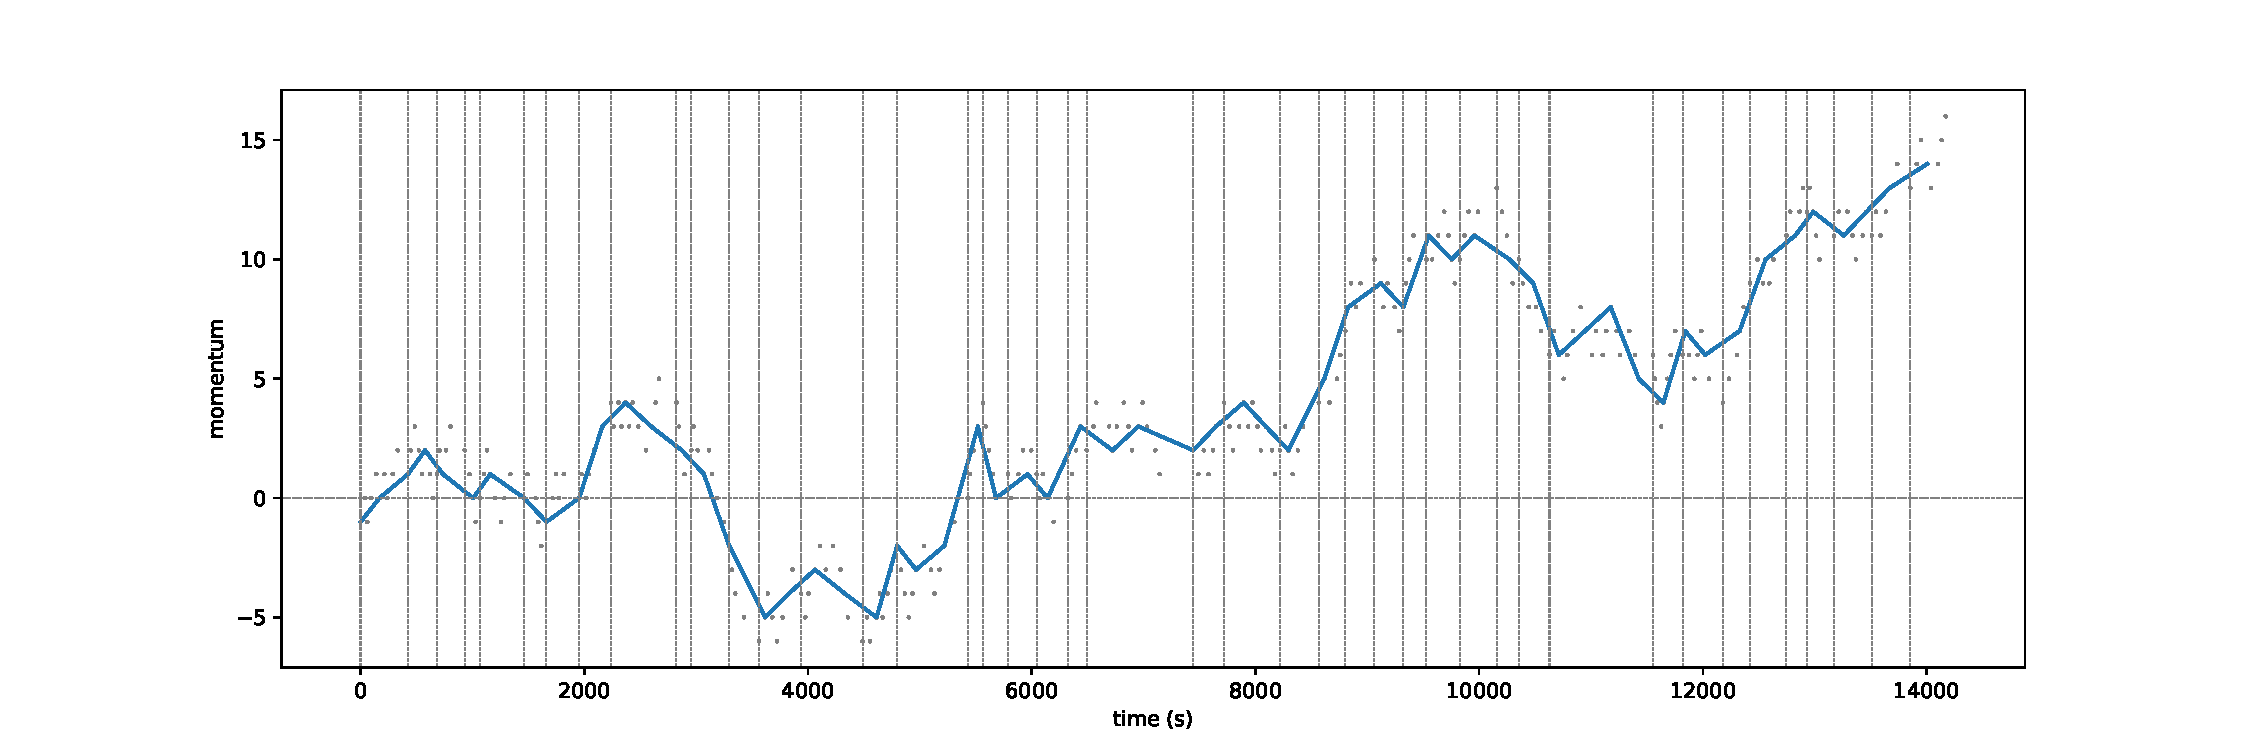
\includegraphics[width=1.0\linewidth]{pics/fig0_0}
		\caption{Global/Cumulative momentum(score difference) graph versus time, 1st match. Dotted lines seperates each game. }
		\label{fig:fig0_0}
	\end{figure}	
	
	\begin{figure}[H]
		\centering
		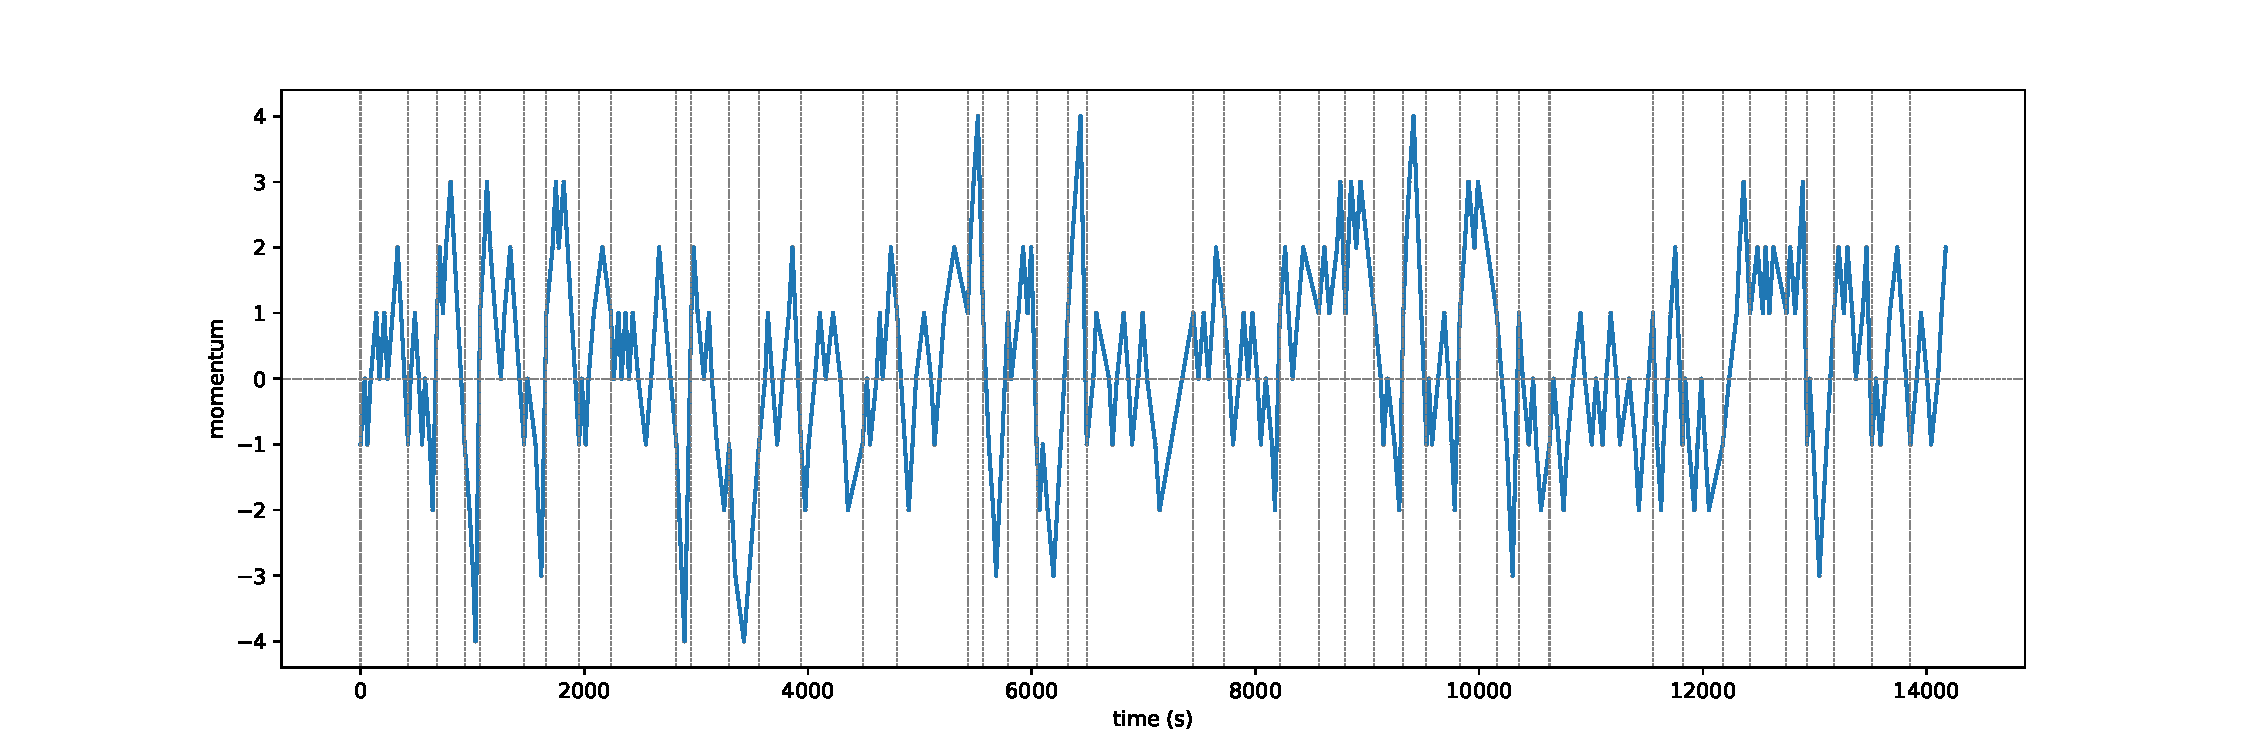
\includegraphics[width=1.0\linewidth]{pics/fig1_0}
		\caption{Momentum(score difference) of each game versus time, 1st match. Dotted lines sepaates each game.}
		\label{fig:fig10}
	\end{figure}
	
	
	We want a model that accounts for more than just score difference. We made 2 considerable additions to the definition of "momentum". 
	\begin{itemize}
		\item Added in "server advantage". Numerous papers have stated that server advantage is an important psychological effect to increase the probability of scoring\cite{Klaassen_1999} \cite{MacPhee_Pollard_2004}, though it alone does not determine the competition outcome. \textbf{We model the effect by adding a "server scoring probability" to whomever is serving.}
		\item Added in "ace". Ace means a server wins a point by serving. This significantly boosts the server's morale. 
	\end{itemize} 
	A modified visualisation shows:
	
	%
	%insert graphs here
	%
	\begin{figure}[H]
		\centering
		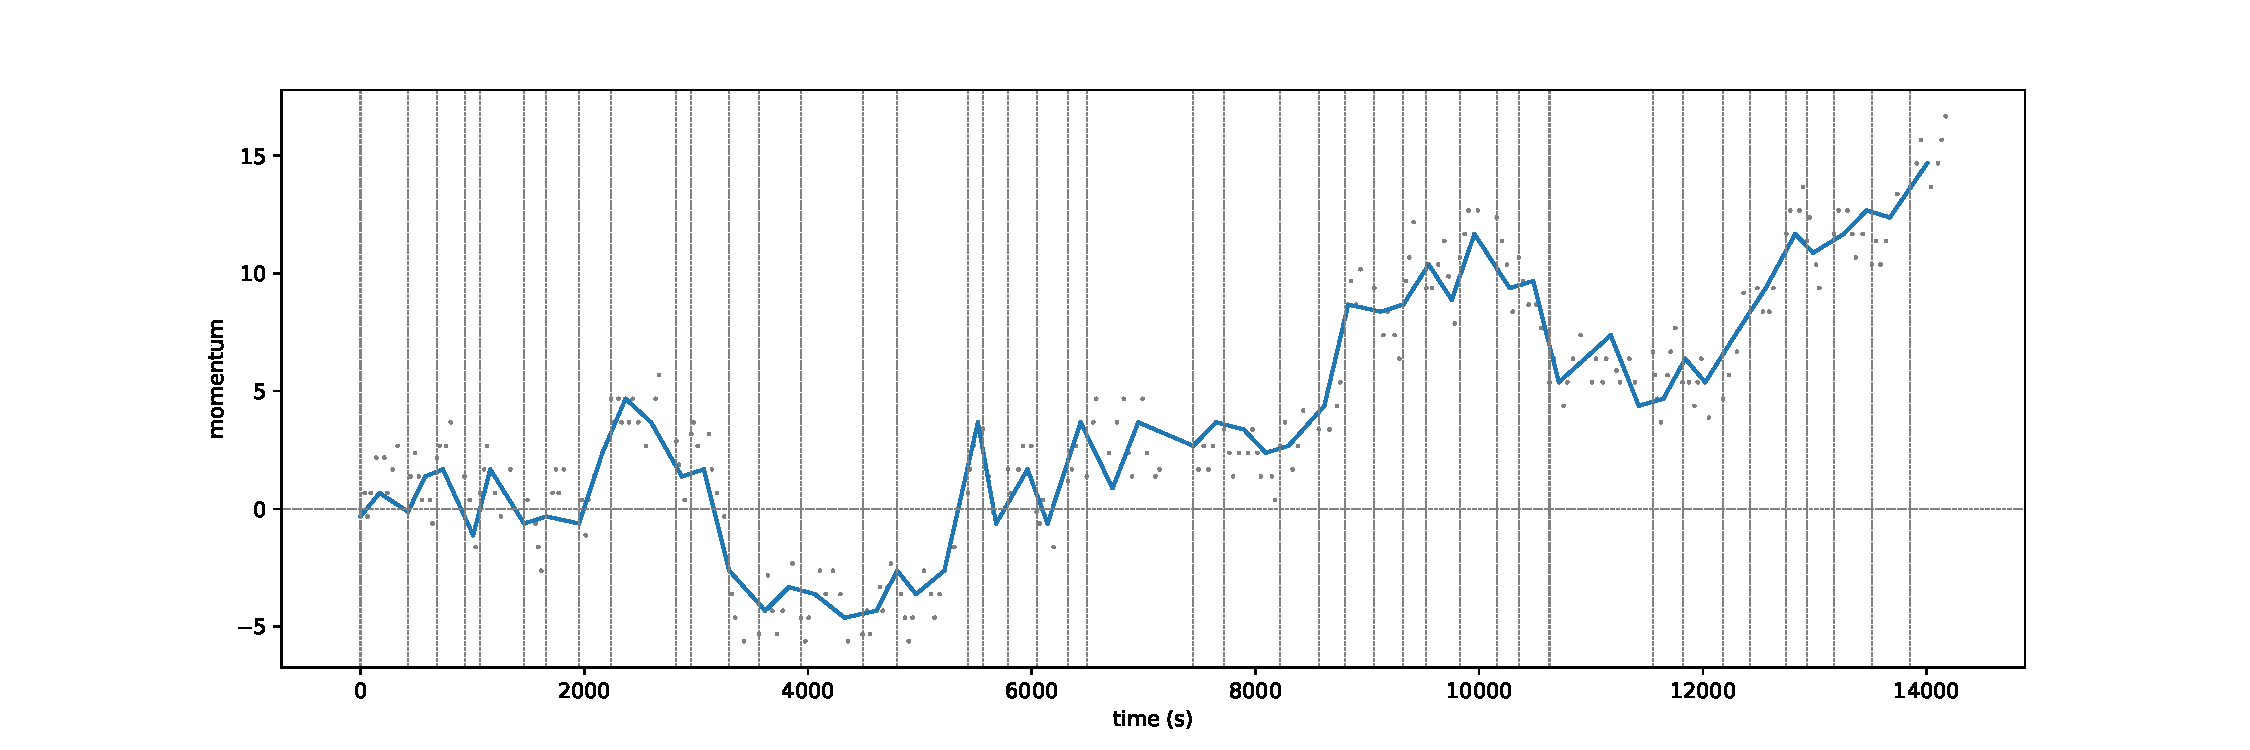
\includegraphics[width=1.0\linewidth]{pics/fig2_0}
		\caption{Modified global/cumulative momentum(score difference) graph versus time, 1st match. Dotted lines seperates each game.}
		\label{fig:fig2_0}
	\end{figure}
	
	\begin{figure}[H]
		\centering
		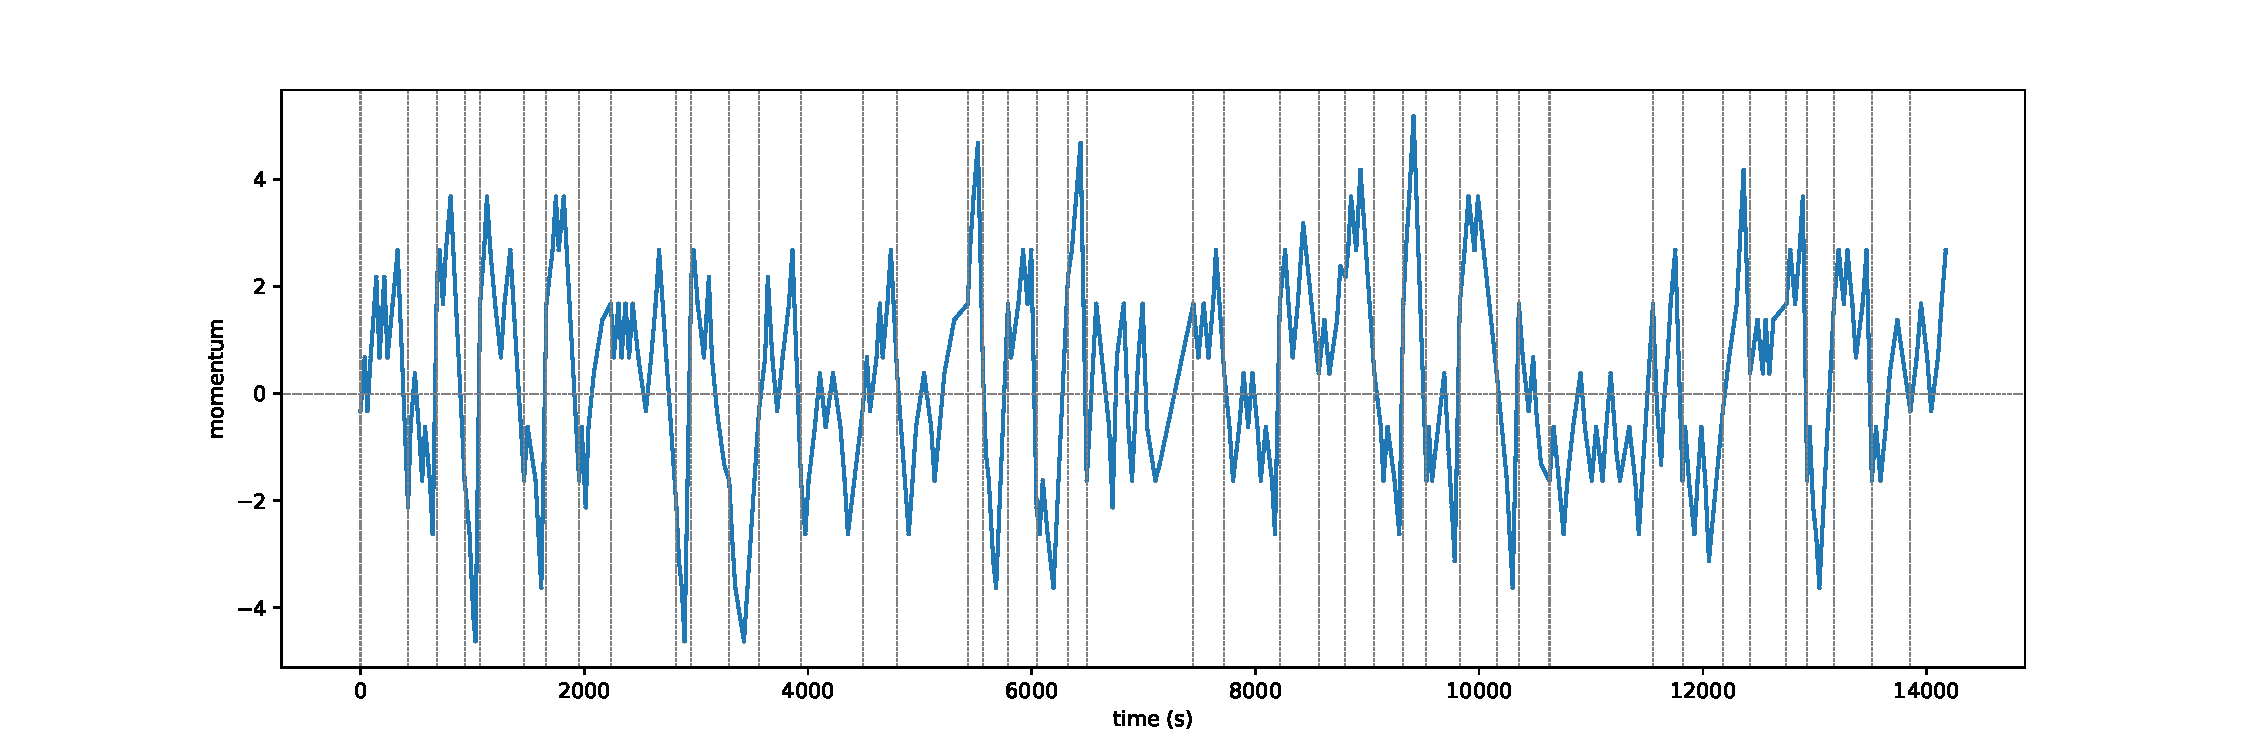
\includegraphics[width=1.0\linewidth]{pics/fig3_0}
		\caption{Modified momentum(score difference) of each game versus time, 1st match. Dotted lines sepaates each game.}
		\label{fig:fig30}
	\end{figure}
	
	We also plotted momentum graphs of the remaining matches. Original data are \color{gray} grey dots \color{black}, and \color{blue}blue trendline \color{black}is drawn based on original data. \color{red} Red lines \color{black} are calculated based on original data.
	
	\begin{figure}[H]
		\centering
		
		% Top subplot
		\begin{subfigure}[b]{\textwidth}
			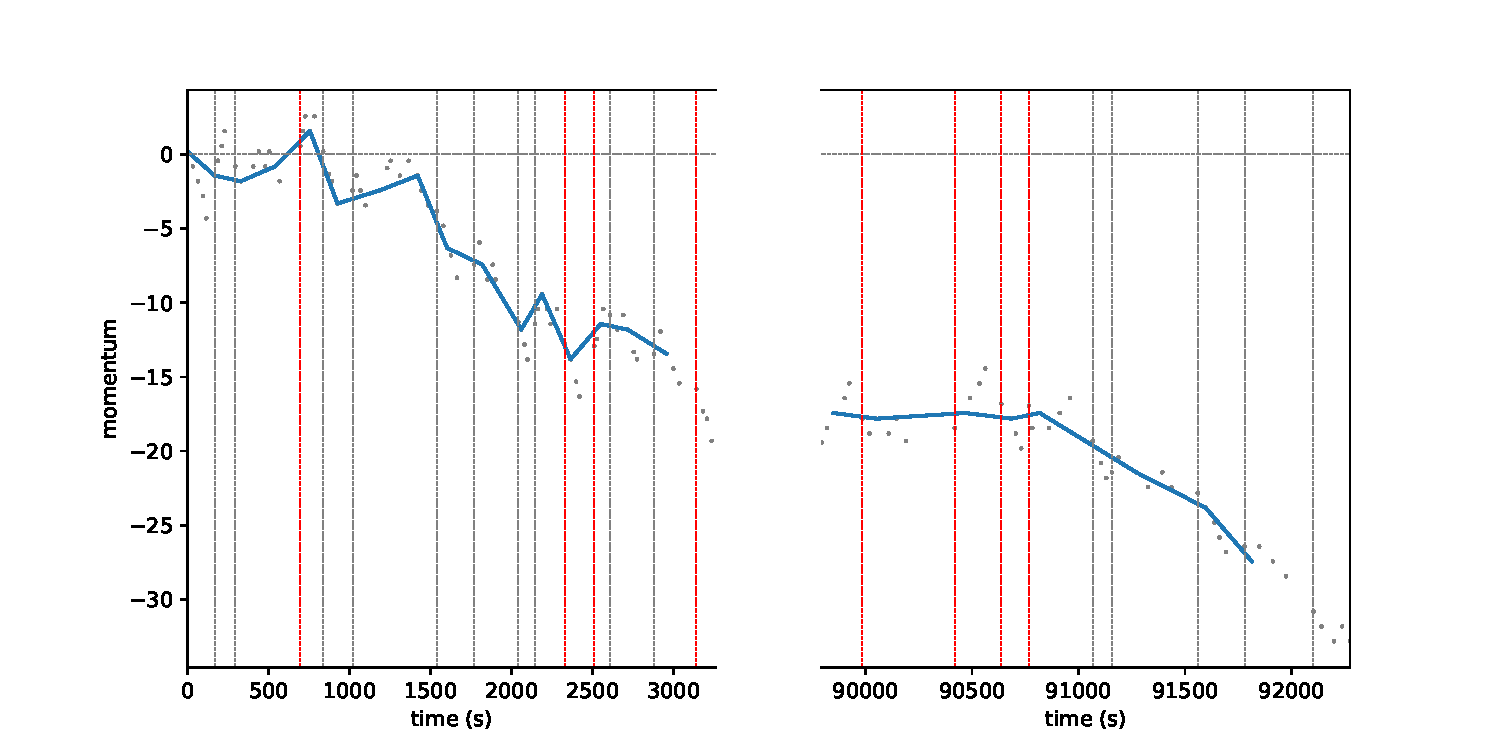
\includegraphics[width=1\linewidth]{pics/fig4_2}
			\caption{Modified global/cumulative momentum(score difference) graph versus time.}
			\label{fig:topfig4_2}
		\end{subfigure}
		
		% Add some space between the figures (optional)
		\vspace{1cm}
		
		% Bottom subplot
		\begin{subfigure}[b]{1.0\textwidth}
			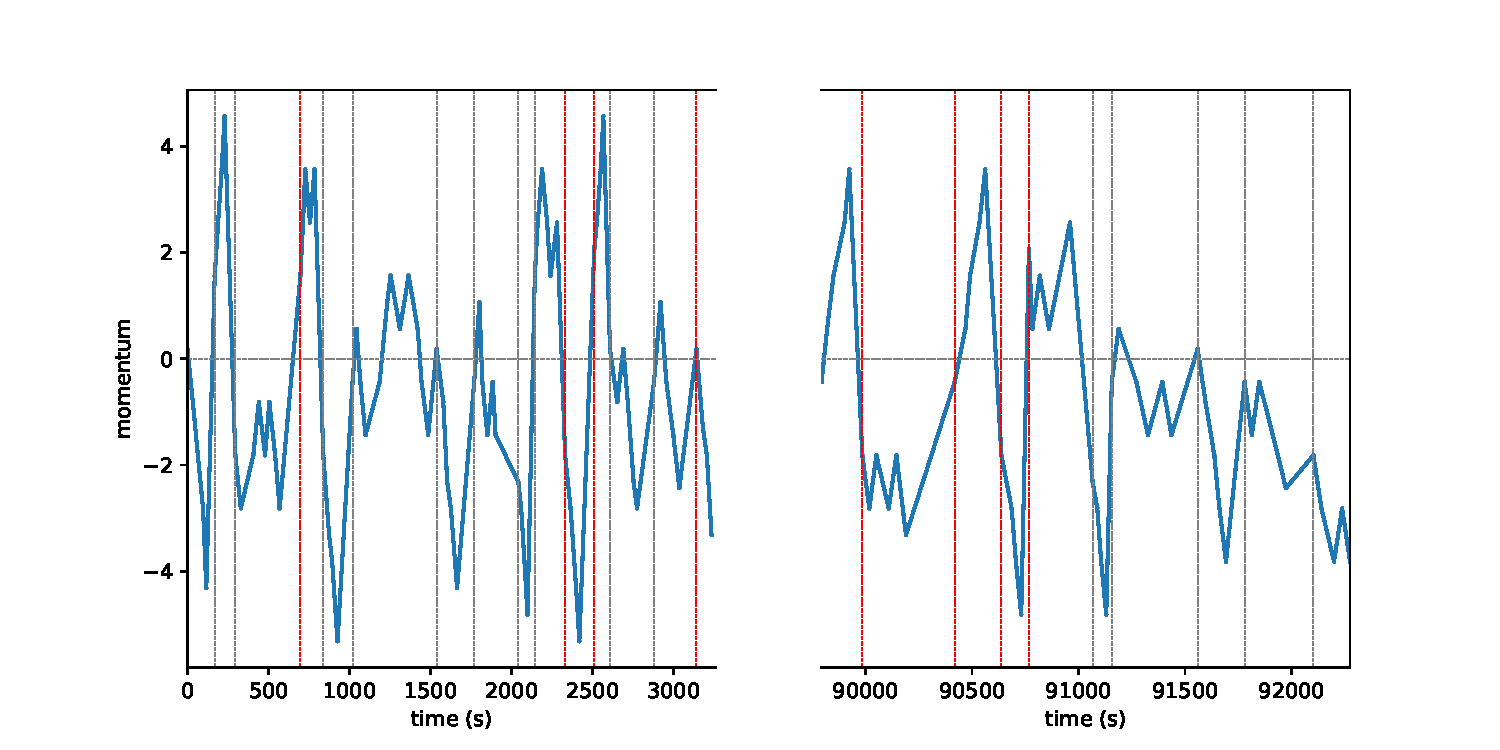
\includegraphics[width=1\linewidth]{pics/fig5_2}
			\caption{Modified momentum(score difference) of each game versus time.}
			\label{fig:bottomfig5_2}
		\end{subfigure}
		
		\caption{2nd match. Dotted lines seperates each game. Dotted red lines indicate swings}
		\label{fig:both_figures2}
	\end{figure}
	
	\begin{figure}[H]
		\centering
		
		% Top subplot
		\begin{subfigure}[b]{\textwidth}
			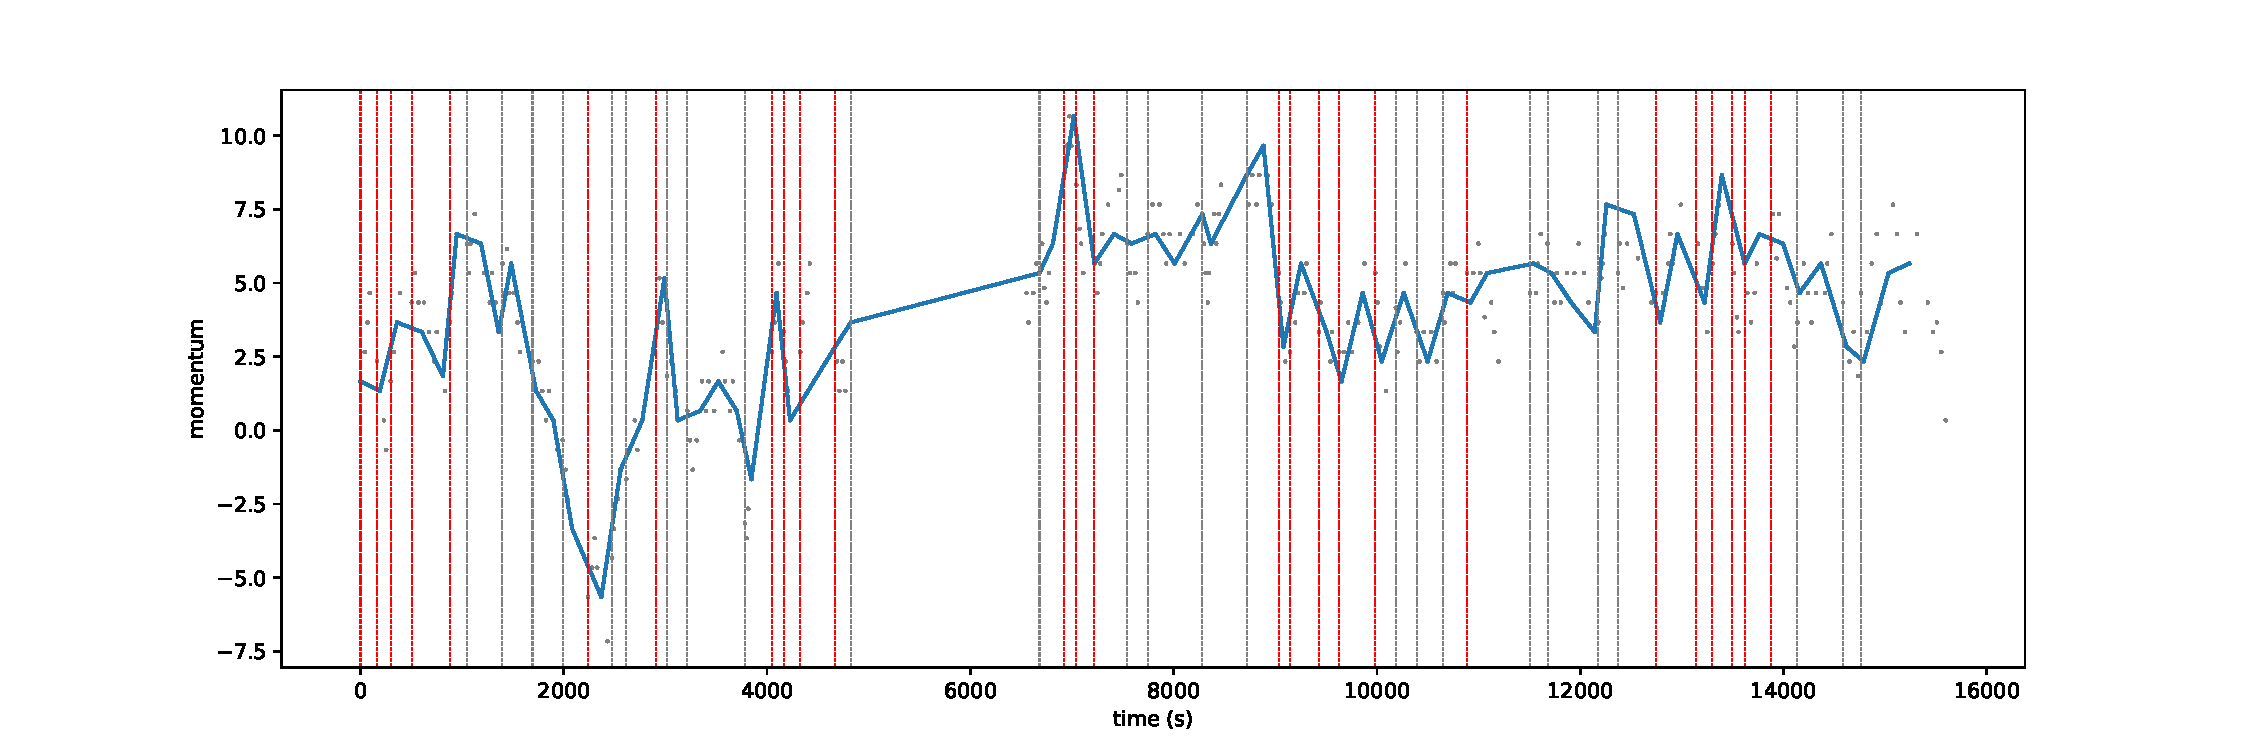
\includegraphics[width=1\linewidth]{pics/fig4_3}
			\caption{Modified global/cumulative momentum(score difference) graph versus time.}
			\label{fig:topfig4_3}
		\end{subfigure}
		
		% Add some space between the figures (optional)
		\vspace{1cm}
		
		% Bottom subplot
		\begin{subfigure}[b]{1.0\textwidth}
			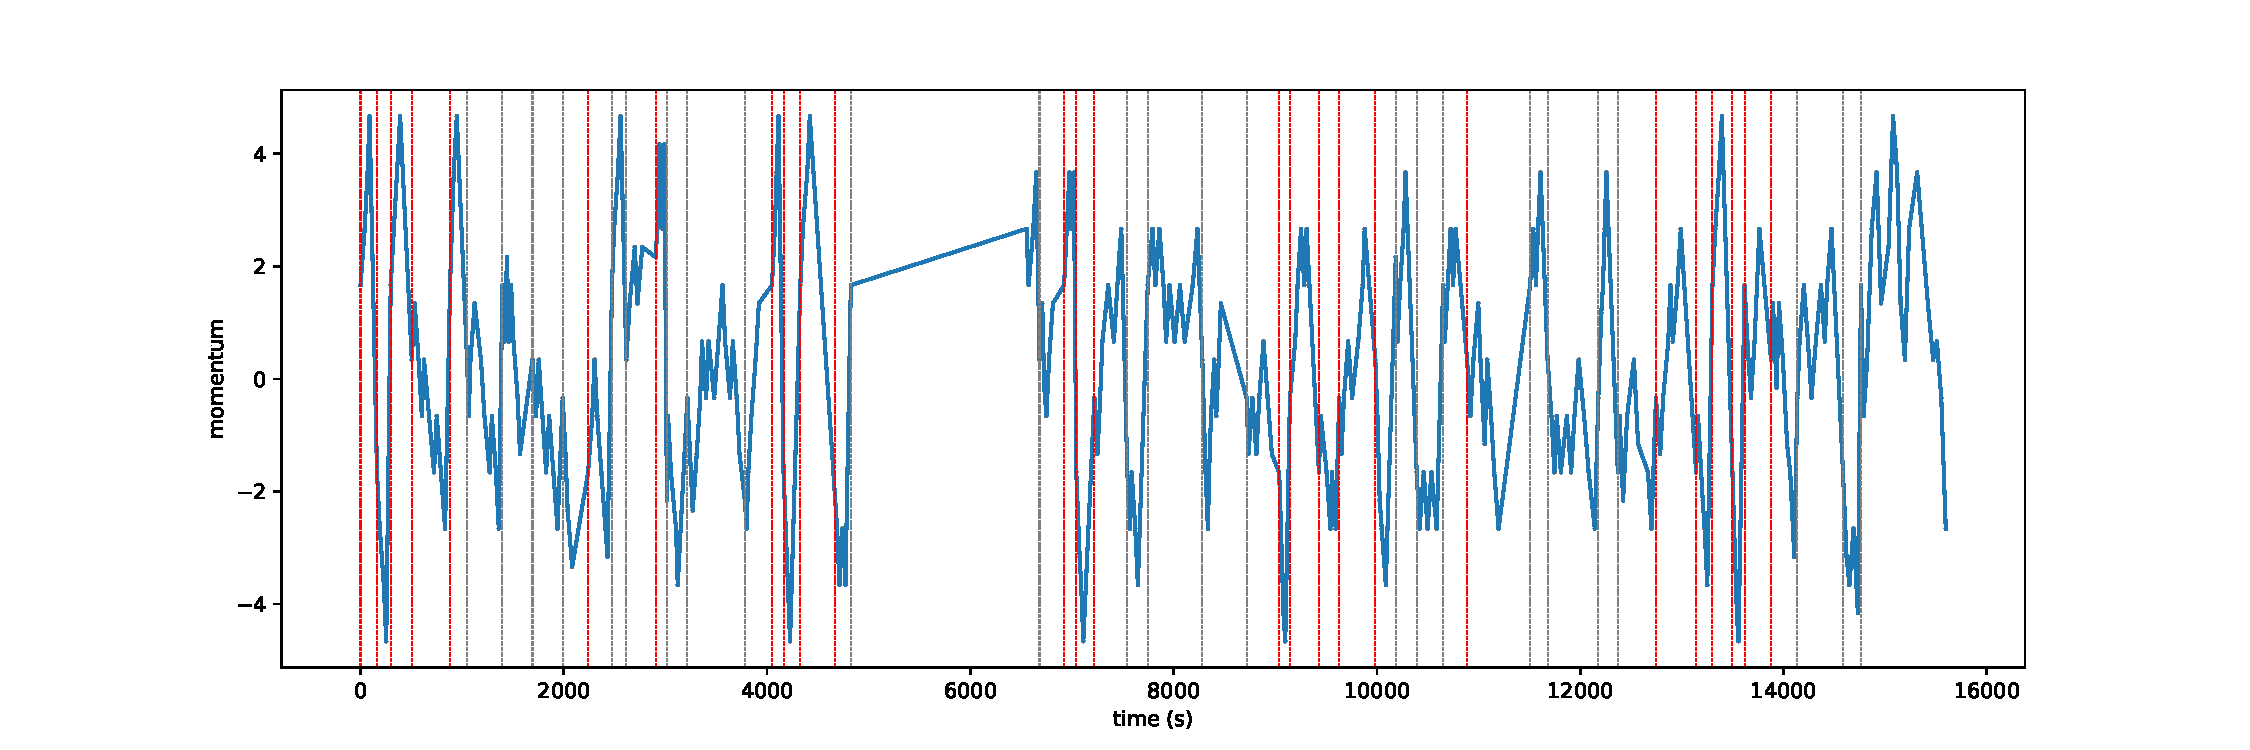
\includegraphics[width=1\linewidth]{pics/fig5_3}
			\caption{Modified momentum(score difference) of each game versus time.}
			\label{fig:bottomfig5_3}
		\end{subfigure}
		
		\caption{3rd match. Dotted lines sepaates each game. Dotted red lines indicate swings}
		\label{fig:both_figures3}
	\end{figure}
	
	\section{Do Swings Happen Randomly?}
	The study of momentum in sports generated great interests among scholars, sports coaches and athletes. The debate is still ongoing--some people do not believen in momentum\cite{Hale_2021}, just like our dear tennis coach.
	
	It was mentioned earlier that the trends of momentum rising and falling reflect performance. We can define the turning point of the rising and falling trends as the inflection point. In each game, by linearly fitting the overall performance of player 1 in the game with the number of balls scored, we can determine the slope that reflects the rising and falling trends. When the performance changes (i.e., when the sign of the slope changes), an inflection point occurs. To filter out the inflection points where the trend changes slowly, only |slope| above a certain threshold are considered as inflection points. These points are marked with red vertical lines on the graph.
	
	In this scenario, we aim to develop a mathematical model to identify turning points in a player's performance trend during a game. The turning points are defined as moments when the trend of performance changes from increasing to decreasing or vice versa, determined by the slope of a fitted line. 
	
	\begin{itemize}
		\item Data Representation
		\begin{itemize}
			\item Let \( t_i \) represent time in the game.
			\item Let \( y_i \) represent the player's score at each \( t_i \).
		\end{itemize}
		\item Linear Regression Model
		\begin{itemize}
			\item We use a simple linear regression model to fit the data points \((t_i, y_i)\).
			\item The linear model is given by \( y = mt + b \), where \( m \) is the slope and \( b \) is the y-intercept. The slope \( m \) indicates the trend of the player's performance. A positive slope implies an increasing trend, while a negative slope indicates a decreasing trend.
			\item To find the best-fit line, we minimize the sum of squared differences between the actual performance scores and the scores predicted by the linear model. The objective is to minimize the Mean Squared Error (MSE), given by:
			\[ MSE = \frac{1}{n} \sum_{i=1}^{n} (y_i - (mt_i + b))^2 \]
		\end{itemize}		
		\item Identifying Turning Points
		\begin{itemize}
			\item A turning point is identified when there is a change in the sign of the slope (from positive to negative or vice versa).
			\item Moreover, to filter out minor fluctuations, a threshold is set for the slope. Only when the absolute value of the slope changes and is greater than a specified threshold (in this case, 0.15) is a turning point acknowledged.
			\item Mathematically, if \( m_{prev} \) and \( m_{current} \) are the slopes of two consecutive segments and \( |m_{current}| > 0.15 \), a turning point is identified when \( \text{sign}(m_{prev}) \neq \text{sign}(m_{current}) \).
		\end{itemize}
	\end{itemize}
	
	Now we have identified all turning points that are actually swings, we need to test for their randomness. We have imposed certain conditions on turning points and the randomness test is as follows:
		
	Let's denote:
	\begin{enumerate}
		\item \( N \) as the total number of games.
		\item \( n_1 \) as the number of games with turning points.
		\item \( n_2 \) as the number of games without turning points.
		\item \( N = n_1 + n_2 \).
		\item \( R \) as the total number of runs (a run is a sequence of consecutive games either all with turning points or all without turning points).
	\end{enumerate}
		
	The expected number of runs (\( E(R) \)) and the variance of the number of runs (\( Var(R) \)) are given by:
	\begin{enumerate}
		\item \[ E(R) = \frac{2n_1n_2}{N} + 1 \]
		\item \[ Var(R) = \frac{2n_1n_2(2n_1n_2 - N)}{N^2(N - 1)} \]
	\end{enumerate}
	
	The test statistic (\( Z \)) is then calculated as:
	\[ Z = \frac{R - E(R)}{\sqrt{Var(R)}} \]
	
	While P-value is given by:
	\[ \text{p-value} = 2P(Z > |z|) \]
	Interpretation	
	\begin{itemize}
		\item If the value of \( Z \) is significantly high or low, it indicates that the turning points are not randomly distributed, suggesting a pattern or trend in the player's performance changes.
		\item A high p-value (usually > 0.05) implies that the turning points are randomly distributed, indicating no specific pattern in performance changes.	
	\end{itemize}
	
	%
	%insert results as table or graph
	\begin{tabular}{|c|c|c|c|}
		\hline
		insert table here&  &  &  \\
		\hline
		&  &  &  \\
		\hline
		&  &  &  \\
		\hline
		&  &  &  \\
		\hline
	\end{tabular}
	%
	\paragraph{Results}
	We have obtained very low p-values, which suggests that swings are not random.
	
	\section{How To Predict Swings?}
	As soon as we have tested the non-randomness of swings, a new question immediately surfaces: can we predict the flow of play? This is very important to sports coaches as it can be used for post-match analysis. Fear not! We have developed a model using deep learning.
	
	But the first step might be the most important step. In order to predict swings, or turning points in a match, we shall first consider the most influential parameters that can have impact on a player’s performance, which can be deduced by the information from the preceding few points. Such parameters are called \textbf{features}.
	
	\subsection{Feature Engineering}
	In our data analysis, the critical parameters that have great impact on dependent variable, or anticipated value shall be regarded as features. Since we have too much data, we shall introduce the method of machine learning. We must feed ML algorithms data in the form of features, to aid in efficient predictions. In our case, predict the performance of each player and if a “swing of momentum” is going to occur.
	
	However, the validity and feasibility of machine learning remarkably depends on the selection and processing of features, due to the different importance of parameters. We shall process the data in a way that generates features that has the greatest correlation on the output. Such step is known as feature engineering, which is the most time-spending but the most critical step in machine learning.
	
	\begin{itemize}
		\item Dependent Variable: Whether a player scores a point (binary 1 or 0), essentially predicting the probability of a player scoring in the next rally.
		\item Independent Variables: Data from all past rallies in the match.
		\item Serve Related Features
		\begin{itemize}
			\item Server Identity: Identifying who is serving, as the server generally has a higher scoring probability.
			\item Ace Balls: Frequency and recent occurrence of ace serves, indicating a higher probability of scoring through aces.
			\item First or Second Serve: First serves generally have a higher win rate.
			\item Serve Direction (Width): Wider serves may lead to higher scoring probabilities.
			\item Serve Depth: Deeper serves may increase the likelihood of scoring.
			\item Serve Speed: Faster serves could correlate with higher scoring probabilities.
			\item Double Faults: Recent double faults could negatively impact the server's scoring probability.
		\end{itemize}
		\item Rally Related Features
		\begin{itemize}
			\item Winning Shots: Recent winning shots can boost a player's scoring probability in the next rally.
			\item Type of Winning Shot: Differentiating between forehand and backhand winning shots.
			\item Net Approaches: Frequency and success rate of net play, indicating a higher scoring probability.
			\item Unforced Errors: Recent unforced errors could decrease a player's scoring probability.
			\item Rally Length: Longer rallies indicating greater physical exertion and potential impact on scoring probability.
			\item Running Distance: Total distance run by each player, indicating physical exertion.
			\item Return Depth: Depth of returns, with deeper returns potentially reducing scoring probability.
		\end{itemize}
		\item Critical Points
		\begin{itemize}
			\item Break Points: Frequency and outcomes of break points, indicating scoring probabilities under high-pressure situations.
			\item Missed Break Points: Impact of missed opportunities on subsequent scoring probability.
			\item Won Break Points: Winning break points could boost a player's scoring probability.
		\end{itemize}
		\item Global Data Features (Reflecting Overall Match Performance)
		\begin{itemize}
			\item Total points, games, sets played.
			\item Match duration.
			\item Total aces, first serve success rate, average serve angle, depth, speed.
			\item Double faults, winning shots, net approaches, and successful net points.
			\item Unforced errors, average return depth, total rally count.
			\item Break point statistics (attained, missed, won).
		\end{itemize}
		\item Local Data Features (Reflecting Recent Performance)
		\begin{itemize}
			\item Duration of recent play, number of serves, aces, first serve success.
			\item Recent serve statistics (angle, depth, speed).
			\item Recent double faults, winning shots, net play frequency, success at the net.
			\item Recent unforced errors, average return depth, rally count.
			\item Recent break point statistics.
			\item Total recent running distance.
		\end{itemize}
	\end{itemize}
	
	\subsection{Regression Model}
	After preparing data, we decided to use a 2-layer linear regression model to train the data. The neural network is a simple feedforward network with two linear layers and a ReLU activation function in between.
	
	\begin{itemize}
		\item Layers:
		\begin{itemize}
			\item First Linear Layer: This layer takes the input vector \( \mathbf{x} \in \mathbb{R}^{n} \) (where \( n \) is the number of features) and transforms it to a hidden vector \( \mathbf{h} \in \mathbb{R}^{m} \) (where \( m \) is the size of the hidden layer, 256 in our case). The transformation is defined as: 
			\[ \mathbf{h} = \mathbf{W}_1 \mathbf{x} + \mathbf{b}_1 \]
			where \( \mathbf{W}_1 \in \mathbb{R}^{m \times n} \) is the weight matrix and \( \mathbf{b}_1 \in \mathbb{R}^{m} \) is the bias vector of the first layer.
			\item ReLU Activation: The ReLU (Rectified Linear Unit) function is applied element-wise to the hidden vector \( \mathbf{h} \). It is defined as:
			\[ \text{ReLU}(h_i) = \max(0, h_i) \]
			for each element \( h_i \) of \( \mathbf{h} \).
			\item Second Linear Layer: This layer maps the hidden vector \( \mathbf{h} \) to the output \( y \in \mathbb{R} \). The transformation is:
			\[ y = \mathbf{W}_2 \mathbf{h} + b_2 \]
			where \( \mathbf{W}_2 \in \mathbb{R}^{1 \times m} \) is the weight matrix and \( b_2 \in \mathbb{R} \) is the bias of the second layer.
		\end{itemize}
		\item  Training:
		\begin{itemize}
			\item Loss Function: The model uses Mean Squared Error (MSE) as the loss function, which for a set of predictions \( \hat{y}_i \) and true values \( y_i \) is given by:
			\[ \text{MSE} = \frac{1}{N} \sum_{i=1}^{N} (\hat{y}_i - y_i)^2 \]
			where \( N \) is the number of samples.
			\item Optimization: The Adam optimizer is used to minimize the loss function. Adam is an adaptive learning rate optimization algorithm that's considered effective for deep learning models.
		\end{itemize}
		\item Prediction: The final model takes an input vector \( \mathbf{x} \), processes it through the layers as described, and outputs a prediction \( y \).		
	\end{itemize}
	
	After 1000 epoches of training, our final result is $\text{Loss}=0.2189$, while $\text{MSE}=0.2287$. 
	
	\begin{figure}[H]
		\centering
		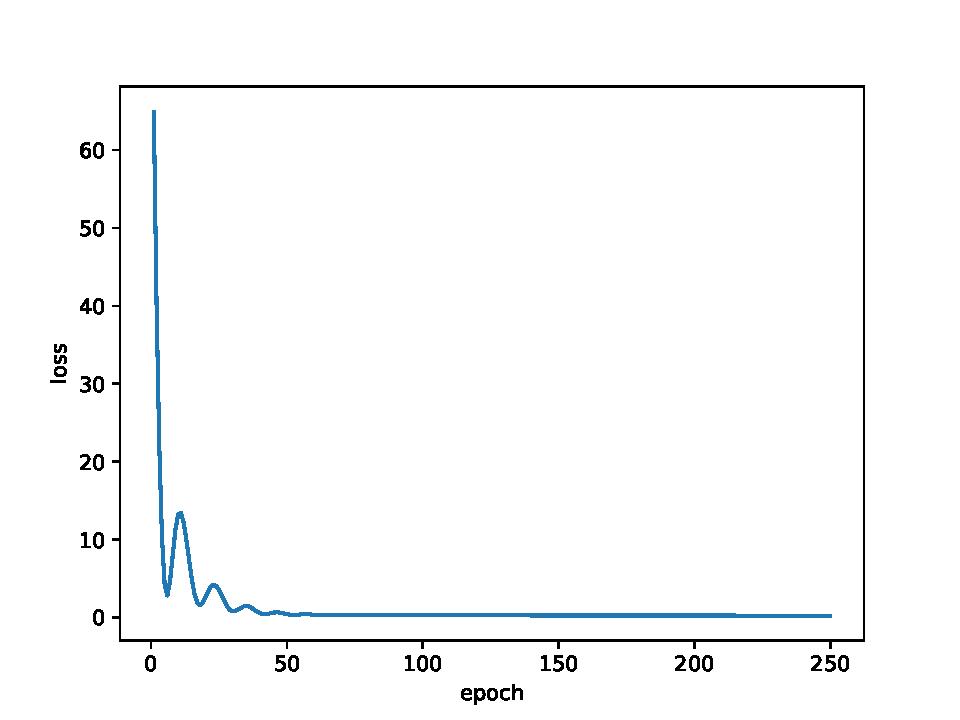
\includegraphics[width=1.0\linewidth]{pics/fig6}
		\caption{Loss versus epoch graph. X-axis is trimmed because loss converges to 0.22 from 250 epoches onwards.}
		\label{fig:fig6}
	\end{figure}
	
	
	Based on this model, we plotted a graph of \color{blue}{actual swings} \color{black} and \color{red}{predicted swings} \color{black}. The accuracy from our model stands around $63.4\%$
	
	
	\begin{figure}[H]
		\centering
		
		% Top subplot
		\begin{subfigure}[b]{\textwidth}
			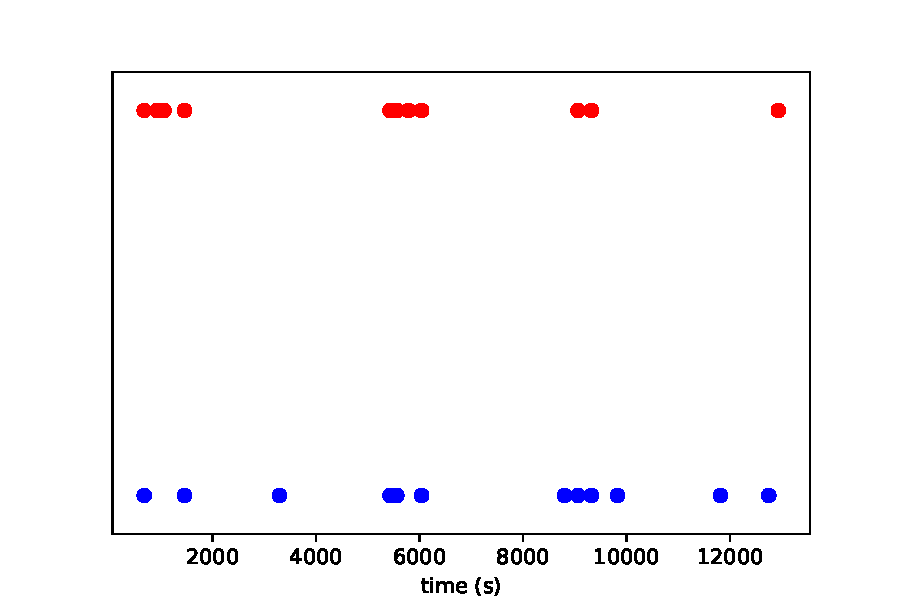
\includegraphics[width=1\linewidth]{pics/fig7_0}
			\caption{1st match}
			\label{fig:topfig7_0}
		\end{subfigure}
		
		% Add some space between the figures (optional)
		\vspace{1cm}
		
		% Bottom subplot
		\begin{subfigure}[b]{\textwidth}
			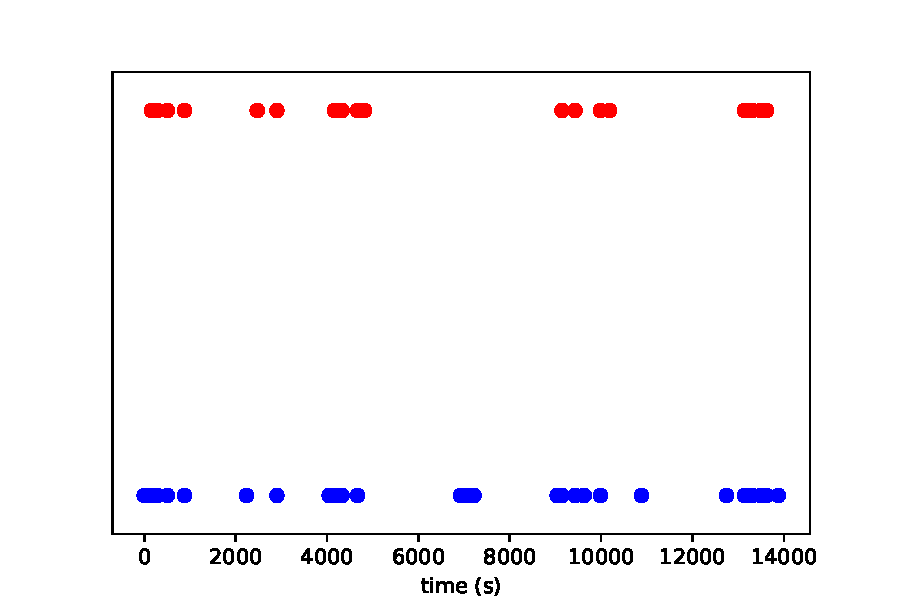
\includegraphics[width=1\linewidth]{pics/fig7_3}
			\caption{3rd match}
			\label{fig:bottom}
		\end{subfigure}
		
		\caption{Predicted swings(red) versus actual swings(blue)}
		\label{fig:both_figures}
	\end{figure}
	
	
	
	\subsection{Classification Model}
	We have tested another deep learning model against our data. The text below outlines how our model works:
	
	\begin{itemize}
		\item Layers:
		\begin{itemize}
			\item Input Layer: Number of nodes equals the number of input features. Let's denote this number as \( n \).
			\item Hidden Layer: Consists of 256 nodes. This layer uses a ReLU (Rectified Linear Unit) activation function.
			\item Output Layer: 2 nodes, corresponding to the classification categories. This layer uses a Softmax activation function for probability distribution.
		\end{itemize}
		\item From Input to Hidden Layer:
		\begin{itemize}
			\item Let \( \mathbf{x} \in \mathbb{R}^{n} \) be the input vector of size \( n \).
			\item The weights connecting the input layer to the hidden layer can be represented as a matrix \( \mathbf{W_1} \in \mathbb{R}^{256 \times n} \).
			\item The bias for the hidden layer is a vector \( \mathbf{b_1} \in \mathbb{R}^{256 \times 1} \).
			\item The output of the hidden layer before activation, \( \mathbf{H} \), is given by  \( \mathbf{H} = \mathbf{W_1} \mathbf{x} + \mathbf{b_1} \), where \( \mathbf{H} \in \mathbb{R}^{256 \times 1} \).
			\item After applying ReLU, the output of the hidden layer becomes \( \mathbf{H'} = \max(0, \mathbf{H}) \), with \( \mathbf{H'} \in \mathbb{R}^{256 \times 1} \).
		\end{itemize}
		\item From Hidden to Output Layer:
		\begin{itemize}
			\item The weights from the hidden layer to the output layer can be represented as a matrix \( \mathbf{W_2} \in \mathbb{R}^{2 \times 256} \).
			\item The bias for the output layer is a vector \( \mathbf{b_2} \in \mathbb{R}^{2 \times 1} \).
			\item The final output before applying softmax, \( Y \), is given by \( Y = \mathbf{W_2} \mathbf{H'} + \mathbf{b_2} \).
			\item The Softmax function is applied to \( Y \) to get the probability distribution over the two classes. If \( Y = [y_1, y_2] \), the softmax function is defined as \( Y = \mathbf{W_2} \mathbf{H'} + \mathbf{b_2} \), where \( Y \in \mathbb{R}^{2 \times 1} \).
		\end{itemize}
		\item Loss Function:
		\begin{itemize}
			\item The model uses Cross-Entropy Loss, which is commonly used in classification tasks. For a single instance with true label \( c \) and predicted probabilities \( p_1, p_2 \), the cross-entropy loss is:
			 \[ \text{Loss} = -\sum_{i=1}^{2} \mathbf{1}(c = i) \log(p_i) \]
			where \( \mathbf{1}(c = i) \) is the indicator function, equal to 1 when \( c = i \) and 0 otherwise.
		\end{itemize}
		\item Optimization:
		\begin{itemize}
			\item Adam Optimizer: This is used for adjusting the weights \( \mathbf{W_1}, \mathbf{W_2} \) and biases \( \mathbf{b_1}, \mathbf{b_2} \) to minimize the loss function. Adam is an adaptive learning rate optimization algorithm that combines the advantages of two other extensions of stochastic gradient descent, namely AdaGrad and RMSProp.
		\end{itemize}
		\item Model Evaluation:
		\begin{itemize}
			\item After training, the model's performance is evaluated by its accuracy on the test dataset. For predicted labels \( \hat{y} \) and true labels \( y \), accuracy is defined as:
			\[ \text{Accuracy} = \frac{\text{Number of Correct Predictions}}{\text{Total Number of Predictions}} = \frac{\sum_{i=1}^{N} \mathbf{1}(\hat{y}_i = y_i)}{N} \]
			where \( N \) is the total number of predictions.
		\end{itemize}
	\end{itemize}
	
	After 300 epoches of training, we achieved an accuracy of $63.96\%$. The loss-epoch diagram is shown below:
		
	\begin{figure}[H]
		\centering
		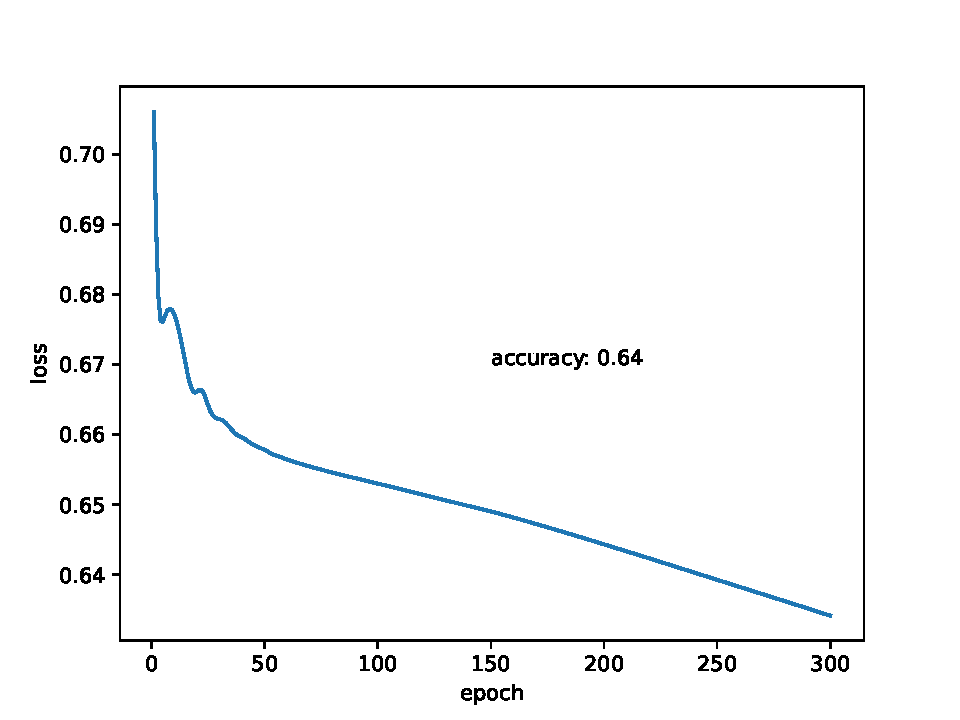
\includegraphics[width=1\linewidth]{pics/fig8}
		\caption{Loss versus epoch graph for classification model. Accuracy is around 0.64}
		\label{fig:fig8}
	\end{figure}
	
	
	
	\bibliography{references}
	\bibliographystyle{plain}
\end{document}